% Template for Cogsci submission with R Markdown

% Stuff changed from original Markdown PLOS Template
\documentclass[10pt, letterpaper]{article}

\usepackage{cogsci}
\usepackage{pslatex}
\usepackage{float}
\usepackage{caption}

% amsmath package, useful for mathematical formulas
\usepackage{amsmath}

% amssymb package, useful for mathematical symbols
\usepackage{amssymb}

% hyperref package, useful for hyperlinks
\usepackage{hyperref}

% graphicx package, useful for including eps and pdf graphics
% include graphics with the command \includegraphics
\usepackage{graphicx}

% Sweave(-like)
\usepackage{fancyvrb}
\DefineVerbatimEnvironment{Sinput}{Verbatim}{fontshape=sl}
\DefineVerbatimEnvironment{Soutput}{Verbatim}{}
\DefineVerbatimEnvironment{Scode}{Verbatim}{fontshape=sl}
\newenvironment{Schunk}{}{}
\DefineVerbatimEnvironment{Code}{Verbatim}{}
\DefineVerbatimEnvironment{CodeInput}{Verbatim}{fontshape=sl}
\DefineVerbatimEnvironment{CodeOutput}{Verbatim}{}
\newenvironment{CodeChunk}{}{}

% cite package, to clean up citations in the main text. Do not remove.
\usepackage{cite}

\usepackage{color}

% Use doublespacing - comment out for single spacing
%\usepackage{setspace}
%\doublespacing


% % Text layout
% \topmargin 0.0cm
% \oddsidemargin 0.5cm
% \evensidemargin 0.5cm
% \textwidth 16cm
% \textheight 21cm

\title{Developmental changes in the ability to draw distinctive visual features
of object categories}


\author{{\large \bf Bria Long} \\ \texttt{bria@stanford.edu} \\ Department of Psychology \\ Stanford University \And {\large \bf Judith E. Fan} \\ \texttt{jefan@stanford.edu} \\ Department of Psychology \\ Stanford University \And {\large \bf Zixian Chai} \\ \texttt{zchai14@stanford.edu} \\ Department of Psychology \\ Stanford University \And {\large \bf Michael C. Frank } \\ \texttt{mcfrank@stanford.edu} \\ Department of Psychology \\ Stanford University}

\begin{document}

\maketitle

\begin{abstract}


\textbf{Keywords:}
object representations; drawings; child development
\end{abstract}

\newcommand{\wrapmf}[1]{#1} 





\section{Introduction}\label{introduction}

While figurative drawings have long provided inspiration for scientists
investigating the representation of object concepts in early life
(Minsky \& Papert, 1972), conclusions about how children express what
they know via drawings have typically come from small-scale laboratory
or observational studies. In fact, while drawings behaviors have been
using as a way to measure children's opinions about social groups
{[}refs{]}, their cognitive abilities \{XX\} or XX, relatively little
work has sought to quantify the changes in the drawings themseves. Those
that have done so have focused largely on the emergence of figurative
drawings in the preschool years {[}cite fenson{]}, documenting the
immensive changes within an individual child. Here we take the opposite
approach -- we seek to create a large-scale, cross-sectional,
naturlaitic database of drwaing behaviors with the hopes of anlayzing
both the consistency and variability in children's drawings. Indeed, we
suspect that there are likely to be large individual differences in
children's ability to draw that may covary with other cultural or
societal factors. there are likely to be large individual and cultural
differences in how children draw,

We thus build a large-scale dataset of children's drawings with the goal
of using children's drawings as a window into how they represent visual
object categories. To do so, we installed a free-standing drawing
station with a digital tablet in a local science museum. So far, this
station has allowed us to collect 13205 drawings for analysis from XX
children, allowing us to examine at scale how drawings of objects change
throughout chilhood. To analyze changes in the visual features of
children's drawings, we capitalize on recent work in recent work that
has validated the use of pre-trained deep convolutional neural network
(DCNN) models to measure high-level perceptual information in drawings
(Fan, Yamins, \& Turk-Browne, 2015) as well as children's drawings
({\textbf{???}}). Higher layers of these models both capture adult
perceptual judgments of object shape similarity (Kubilius, Bracci, \& Op
de Beeck, 2016) and predict neural population responses in categories
throughout object-selective cortex (Yamins et al., 2014). Thus, features
learned by these models provide a principled choice of basis for
extracting perceptual features useful for inferring object identity from
children's drawings.

Here, we begin the analysis of this dataset with three main goals. In
recent work ({\textbf{???}}) with a smaller sample of drawings, the
recognizaiblty of children's drawings increased across childhood, and
these changes in recognizabilty were paralleled by changes in the
representations of children's drawings in these high-level visual
features Thus, here we first aim to both replicate and unify these
findings by directly (1) examining if the intended category of
children's drawings can be read out from these high-level features using
a linear classifier and (2) if classifier performance increases with
age. Second, given that motoric abilities also increase across this age
range, we developmetrics for evaluating tracing abilities and apply
these to examine the relationship children's tracing performance and
classifier performance. Finally, to give insight into the kinds of
changes that may explain this age-related gain in recognizability, we
explore how the representations of children's drawings in high-level
visual feature space changes across childhood.

\section{Methods}\label{methods}

\subsubsection{Drawing Task Procedure}\label{drawing-task-procedure}

We implemented a web-based drawing game in HTML/Javascript using the
paper.js library and collected drawings using a touchscreen tablet on
the floor of the museum; each participant sat in front of this
table-mounted touchscreen display. At the beginning of each session,
children completed two tracing trials (square, complex shape) and one
copying trial (square or circle), designed to assess their ability to
coordinate their motor movements (see Tracing Evaluation). After the
tracing trails, on each trial, a video of an experimenter verbally
prompted children to draw a particular object category (e.g., ``What
about a dog? Can you draw a dog?''); children had up to 30 seconds to
complete their drawings with their fingers. The timimg and position of
each stroke was saved to an online database and permitting the
calculating of the overall time spent drawing, the amount of ink used,
and the number of strokes made as basic covariates.

Stimuli were videos an experimenter verbally referring to 23 common
object categories: house, couch, chair, airplane, bike, car, boat,
train, bear, cat, rabbit, dog, sheep, bird, frog, fish, person, tree,
bowl, phone, cup, scissors, and key. Participants could draw a maximum
of 8 stimuli per session, which were part of the drawing station for
several months at a time. These categories were chosen to be likely
familiar to children, to cover a wide range of superordinate categories,
and to vary in the degree to which they are commonly practiced in
drawings by children.

\subsubsection{Data Filtering}\label{data-filtering}

Raw drawing data (N=15594 drawings) were conservatively screened for
task compliance using a combination of manual and automated procedures
(i.e., excluding blank drawings, pure scribbles, and drawings containing
words), resulting in the exclusion of 23.8\% of drawings. We adopted
conservative screening procedures to ensure that any age-related trends
we observed were not due to differences in task compliance across age.
Similarily, while viewing a first subset of the drawings, we noticed
many very stylized drawings by our youngest participants (2-year-olds);
thus, in later versions of the drwaing station, we also presented
participants with an optional survey to indicate if either another child
or an adult had also drawn during the session; all drawings where
intererence was reported were excluded from analyses (XX\% of valid
sessions in subset).

\subsubsection{Participants}\label{participants}

After filtering, we analyzed data from N=1259 children who were on
average 5.44 years of age (range 2-10 years); participants age was
self-reported and no other identifying information was collected.

\begin{CodeChunk}
\begin{figure}[H]

{\centering 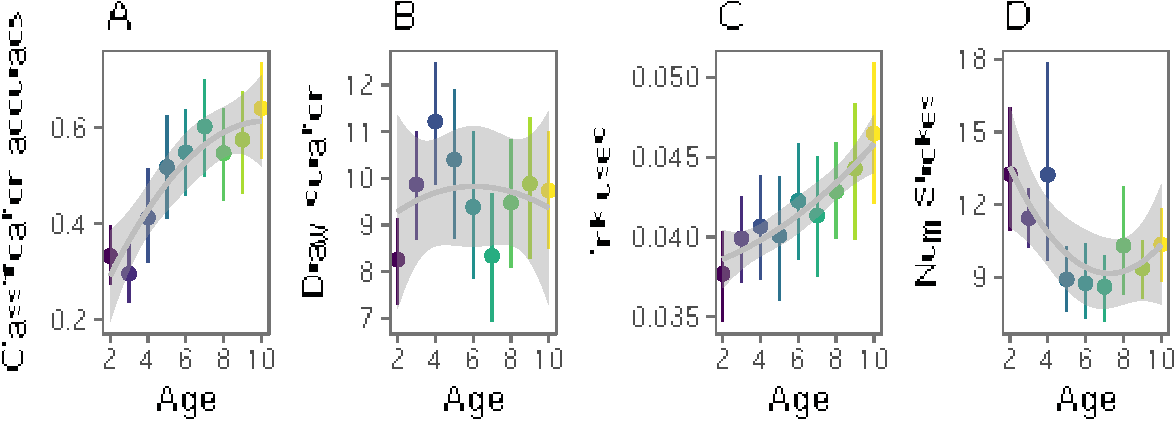
\includegraphics{figs/unnamed-chunk-1-1} 

}

\caption[Leave-one-out classification accuracy (A), the amount of time spent drawing in seconds (B), the amount of ink used (i.e., mean intensity of the drawings) (C), and the number of strokes used (D) are plotted as a function of children’s age]{Leave-one-out classification accuracy (A), the amount of time spent drawing in seconds (B), the amount of ink used (i.e., mean intensity of the drawings) (C), and the number of strokes used (D) are plotted as a function of children’s age. }\label{fig:unnamed-chunk-1}
\end{figure}
\end{CodeChunk}

\begin{CodeChunk}
\begin{figure*}[h]

{\centering 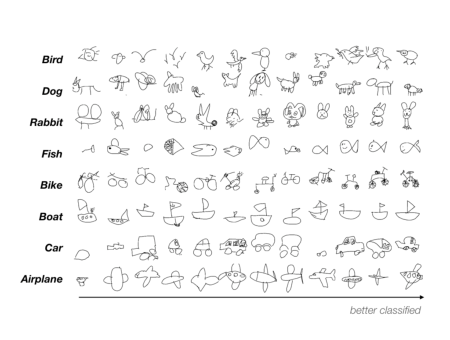
\includegraphics[width=1\linewidth]{figs/exampleDrawings-1} 

}

\caption[Example drawings made by children ages 4-10 of several object categories]{Example drawings made by children ages 4-10 of several object categories.}\label{fig:exampleDrawings}
\end{figure*}
\end{CodeChunk}

\subsubsection{Tracing Evaluation}\label{tracing-evaluation}

\subsubsection{Deep Convolutional Neural Network
Model}\label{deep-convolutional-neural-network-model}

We used a standard, pre-trained implementation of the VGG-19
architecture (Simonyan \& Zisserman, 2014) to extract features from
sketches at the last full-connected layer of the network known to
support category recognition in both photos. Eeach image elicits a
pattern of feature activations (here, 4096 features per image). Features
were normalized across the entire image set before analysis (but not
normalized within each category or age group). These features form a
common basis for representing complex shape similarity -- including the
presence of diagnostic object parts (e.g., legs, handles) -- and a basis
from which object identity can be easily derived (Kubilius et al.,
2016).

\subsubsection{Logistic Regression
Classifier}\label{logistic-regression-classifier}

We used the features extracted by VGG-19 to train a 23-way logistic
regression model under leave-one-out cross-validation to estimate the
recognizability of drawings produced by children in each age group;
importantly, this model had no information about the age of the drawer
but was randomly under sampled such that there were an equal number
images for each of the 23 categories. This iterative modeling procedure
yielded a both a binary classification score for each image as well as
the probability that each image was assigned to each category in the
dataset.

\subsubsection{Model Fitting}\label{model-fitting}

We anticipated that their drawings may also vary along other dimensions
more directly related to the motor production demands of the task, such
as the amount of time spent drawing, the number of strokes used, and
amount of ink (i.e., mean pixel intensity of sketch). In order to assess
whether children's ability to produce recognizable drawings increased
with age, independent of these low-level covariates, we fit a
generalized linear mixed-effects model, with scaled age (specified in
years), drawing duration, amount of ink used, and number of strokes as
fixed effects, and with random intercepts for each individual child and
object category. The dependent variable was whether the linear
classifier was able to correctly classify the drawing or the probability
assigned to the target category

\subsubsection{Feature Space Metrics}\label{feature-space-metrics}

To explore changes in the visual features of these drawings, for each
age group and object category, we computed the mean feature vector
(category center), as well as the root-mean-squared deviation of
drawings from their category center using eucildean distance (category
dispersion). For each pair of object categories within each age, we used
these two metrics to compute a high-dimensional analogue of d-prime
(distinctiveness). The overall change in the size of the feature space
was measured by computing the the root-mean-squared deviation of
category-centers from the overall grand mean of this feature space
(overall dispersion).

For representational similarity analysis, the Pearson correlation
distances between these average feature vectors for each category was
computed (Kriegeskorte, Mur, \& Bandettini, 2008) to contruct 23x23
representational dissimilarity matrices (RDM); these RDMs provide a
compact description of the layout of these cateogries in the
high-dimensional feature space. Following Kriegeskorte et al. (2008), we
computed the Spearman rank correlations between the RDMs between at each
age vs.~the oldest children in our sample (10-year-olds). Estimates of
standard error for the both the Spearman correlation between RDMs, were
generated by jackknife resampling of the 23 object categories.

\section{Results}\label{results}

Overall, we found that the model's classification accuracy increased
with age (see Figure X). Further, the average probability assigned to
the target category increase with age even when restricting our analyses
to drawings that were correctly classified, suggesting that
classification confidence also increases with age (see Figure X)

Next, we examined the contributions of basic task-covariates (e.g.,
number of strokes, ink used, time spent drawing) as well as tracing
performance to these gains in classification (see Figure XX).
\emph{Briefly, tracing performance was evaluated by terms that take into
account both the spatial error and shape error in XX metric; this metric
was validated on a sample of human-judgements on 2000 tracings (r=XX,
p=XX, \ldots{}).} Our mixed-effects model revealed that both the
classification accuracy of drawings as well as classification confidence
(for correct drawings only) reliably increased with age when accounting
for these covariates --- tracing ability, the amount of time spent
drawing, the number of strokes, and total ink used and accounting for
variation across object categories and individual children.
(classification accuracy: \(\beta\) = 0.53, SE = 0.039, Z = 13,
classification confidence: \(\beta\) = 0.53, SE = 0.039, Z = 13 ). All
model coefficients can be seen in Table 1.

To investigate the underlying source of these changes in
recognizability, we examined changes in this feature space across age.
First, the degree to which drawings elicited robust, variable responses
in this feature space increased with children's age, suggesting that
older children's drawings may simply contain more detailed and more
variable high-level visual features (stats). Relatedly, we also found
that the overall distnace between category centers and the average of
the feature space increased wiht age, suggestiong an overall expnaion of
the feature space with age (stats) Second, as in prior work, we found
that the correlation bewteen RDMs generally increased with age,
suggesting that part of the gain in category classificaiton across age
can be attributed to shifts in the relative positions of the category
center (stats.) Finally, we also observed a small but consistent
decrease in within-category dispersions decreased with age, as well as
an overall increase in visual discriminability (i.e., higher-dimensional
analog of d-prime) (mean d-prime across all category pairs, 2-yrs,
M=0.3, 3-yrs, M=0.27, 4-yrs, M=0.35, 5-yrs, M=0.42, 6-yrs, M=0.45,
7-yrs, M=0.49, 8-yrs, M=0.49, 9-yrs, M=0.51).

\subsubsection{Representational Similarity
Analyses}\label{representational-similarity-analyses}

\section{General Discussion}\label{general-discussion}

\subsection{Findings: changes in VGG features directly related to gains
in classificatino in large-scale dataset, controlling for basic tracing
abilities as well as basic motor covariates. Suggests that object
children are better able to produce these distinctive features for
recognition, perhaps paralleling their emerging perceptual and
categorization abilities
{[}cite{]}}\label{findings-changes-in-vgg-features-directly-related-to-gains-in-classificatino-in-large-scale-dataset-controlling-for-basic-tracing-abilities-as-well-as-basic-motor-covariates.-suggests-that-object-children-are-better-able-to-produce-these-distinctive-features-for-recognition-perhaps-paralleling-their-emerging-perceptual-and-categorization-abilities-cite}

\subsection{Next steps: relate production and recognition
(animalgame)}\label{next-steps-relate-production-and-recognition-animalgame}

\subsection{Understand which features of objects drive changes in
recognition, and how these are related to
memory}\label{understand-which-features-of-objects-drive-changes-in-recognition-and-how-these-are-related-to-memory}

\subsection{Understand relative contributions of cultural conventions
(and item
effets)}\label{understand-relative-contributions-of-cultural-conventions-and-item-effets}

\vspace{1em}

\fbox{\parbox[b][][c]{7.3cm}{\centering All data and code for these analyses are available at\ \url{https://github.com/brialorelle/kiddraw}}}
\vspace{1em}

\section{Acknowledgements}\label{acknowledgements}

???? We thank members of Stanford Language and Cognition lab. This work
was funded by an NSF SPRF-FR Grant \#1714726 to BLL and a Jacobs
Foundation Fellowship to MCF.

\section{References}\label{references}

\setlength{\parindent}{-0.1in} \setlength{\leftskip}{0.125in} \noindent

\hypertarget{refs}{}
\hypertarget{ref-fan2015common}{}
Fan, J. E., Yamins, D., \& Turk-Browne, N. B. (2015). Common object
representations for visual recognition and production. \emph{Proceedings
of the 37th Proceedings of Annual Conference of the Cognitive Science
Society.}

\hypertarget{ref-kriegeskorte2008RSA}{}
Kriegeskorte, N., Mur, M., \& Bandettini, P. (2008). Representational
similarity analysis--connecting the branches of systems neuroscience.
\emph{Frontiers in Systems Neuroscience}, \emph{2}.

\hypertarget{ref-kubilius2016deep}{}
Kubilius, J., Bracci, S., \& Op de Beeck, H. P. (2016). Deep neural
networks as a computational model for human shape sensitivity.
\emph{PLoS Computational Biology}, \emph{12}(4), e1004896.

\hypertarget{ref-minsky1972artificial}{}
Minsky, M., \& Papert, S. A. (1972). Artificial intelligence progress
report.

\hypertarget{ref-simonyan2014very}{}
Simonyan, K., \& Zisserman, A. (2014). Very deep convolutional networks
for large-scale image recognition. \emph{ArXiv Preprint
ArXiv:1409.1556}.

\hypertarget{ref-yamins2014performance}{}
Yamins, D., Hong, H., Cadieu, C. F., Solomon, E. A., Seibert, D., \&
DiCarlo, J. J. (2014). Performance-optimized hierarchical models predict
neural responses in higher visual cortex. \emph{Proceedings of the
National Academy of Sciences}, \emph{111}(23), 8619--8624.

\end{document}
